In Fig. \ref{fig:dt} the decision tree structure can be found. It is important
to remark that this tree did not consider any of the discrete variables is
critical to separate the data. This was also highlighted by the SVMs, as only
the dimension that used Emotional Socialization was important to separate the
data. One crucial feature of decision trees is that they create an intuitive
structure for the dataset; in this manner, it confirms the behavior already
established for the SVM's and presents a hierarchy between the variables.

\begin{figure}
  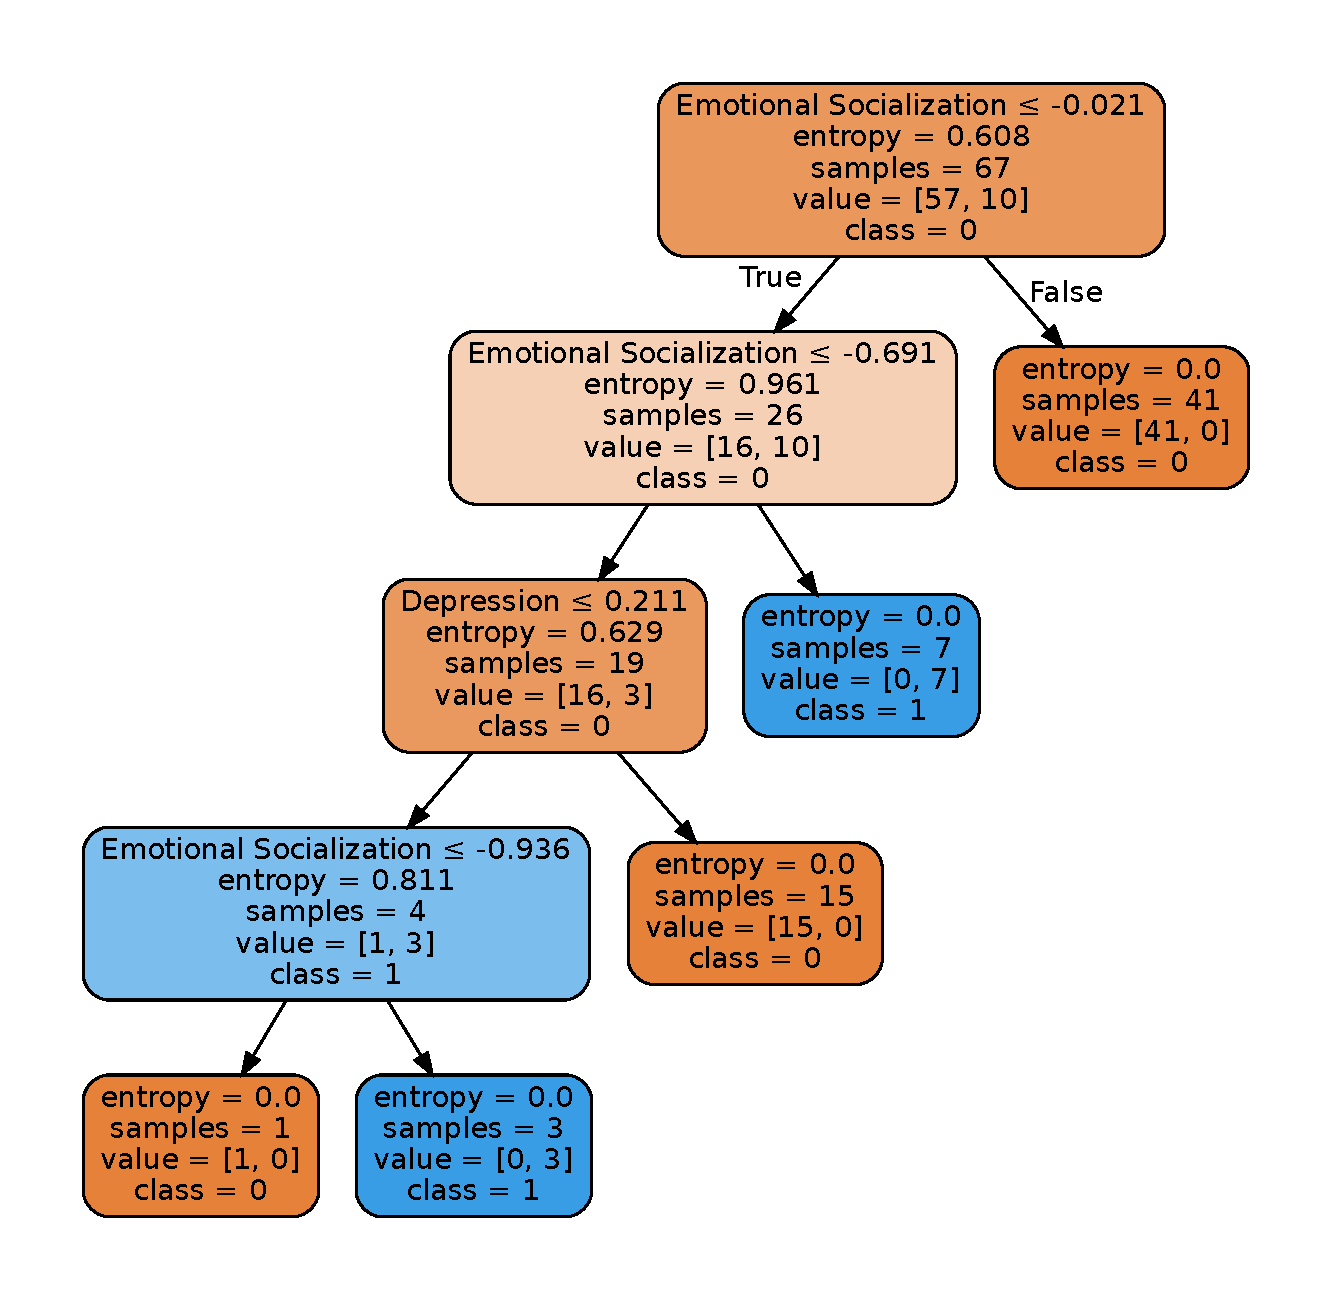
\includegraphics[width=\columnwidth]{figs/tree-graph.pdf}
  \caption{Decision tree.}
  \label{fig:dt}
\end{figure}

In Table \ref{tab:DT} it is seen that the performance of this machine was
superior to all of the other machines in terms of specificity and sensitivity.
In this manner, this highlights that the other discrete variables may not be as
important and they may present difficulties for other machines that try to take
into account all of the variables.

\begin{table}
  \centering
  \caption{Performance scores for DT.}
  \label{tab:DT}
  \begin{tabular}{ccc}
    \hline
    \textbf{Set} & \multicolumn{1}{c}{\textbf{Sensitivity}} & \multicolumn{1}{c}{\textbf{Specificity}} \\ \hline
    Training & 1 & 1 \\
    Testing & 0.5 & 1 \\
    Validation & 0.75 & 1 \\ \hline
  \end{tabular}
\end{table}

Lastly, in Fig \ref{fig:dts} the behavior of the tree is seen. It is noticed
that the tree was apple to learn the best at classifying the class 1 separating
the space between the sides and the middle. Furthermore, it did not present any
important value for the other variables.

\begin{figure*}
  \centering
  \begin{subfigure}[b]{0.32\textwidth}
    \centering 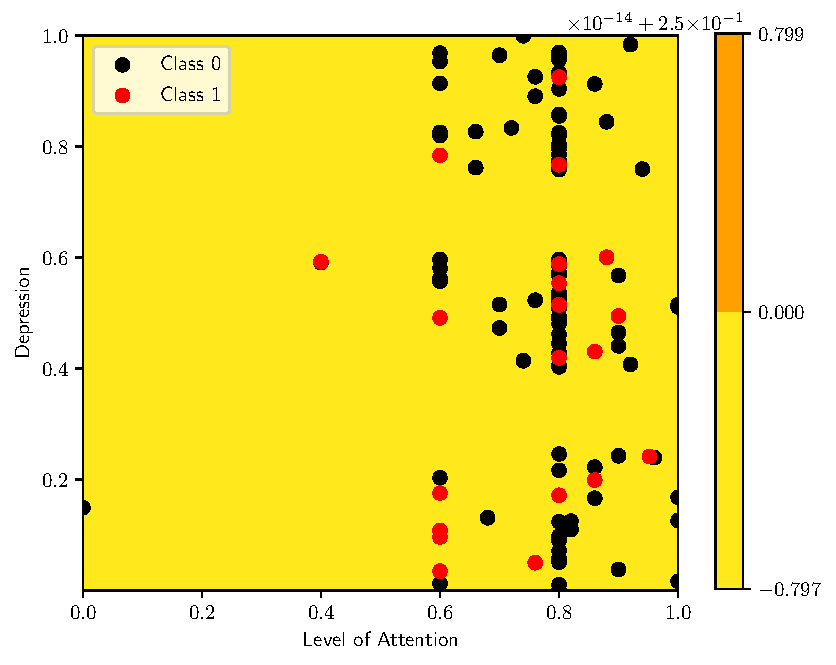
\includegraphics[width=\textwidth]{figs/tree-contour-0-3.pdf}
    \caption{}
  \end{subfigure}
  \begin{subfigure}[b]{0.32\textwidth}
    \centering 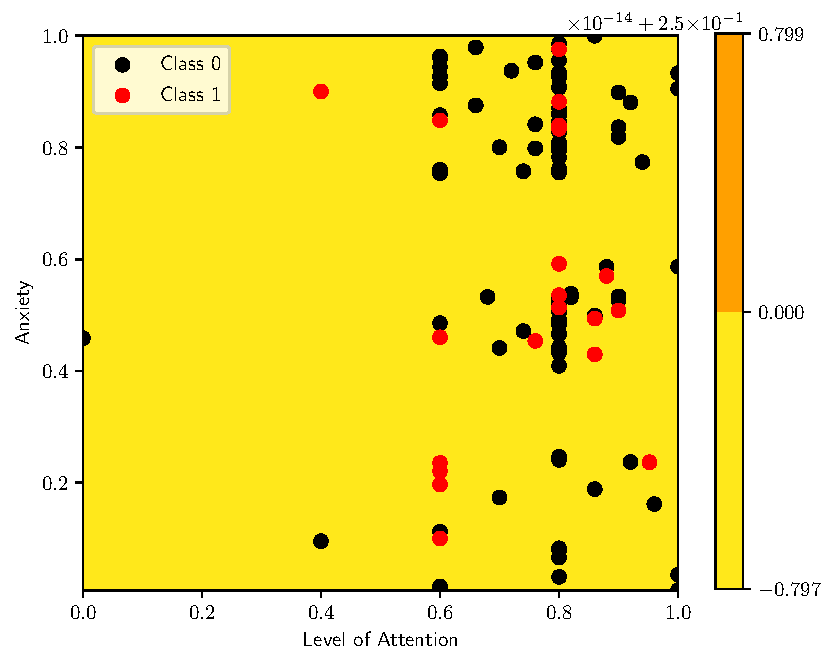
\includegraphics[width=\textwidth]{figs/tree-contour-0-4.pdf}
    \caption{}
  \end{subfigure}
  \begin{subfigure}[b]{0.32\textwidth}
    \centering 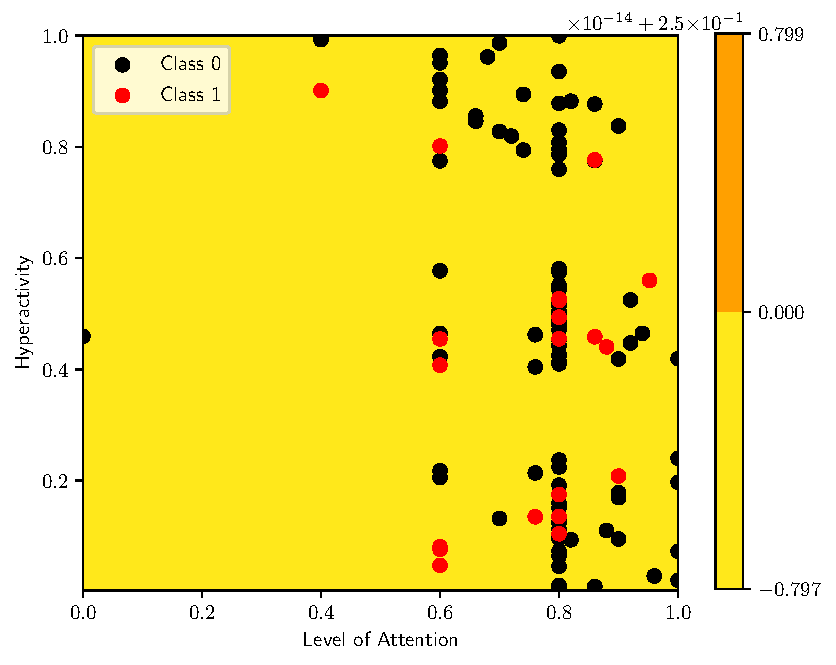
\includegraphics[width=\textwidth]{figs/tree-contour-0-5.pdf}
    \caption{}
  \end{subfigure}

  \begin{subfigure}[b]{0.32\textwidth}
    \centering 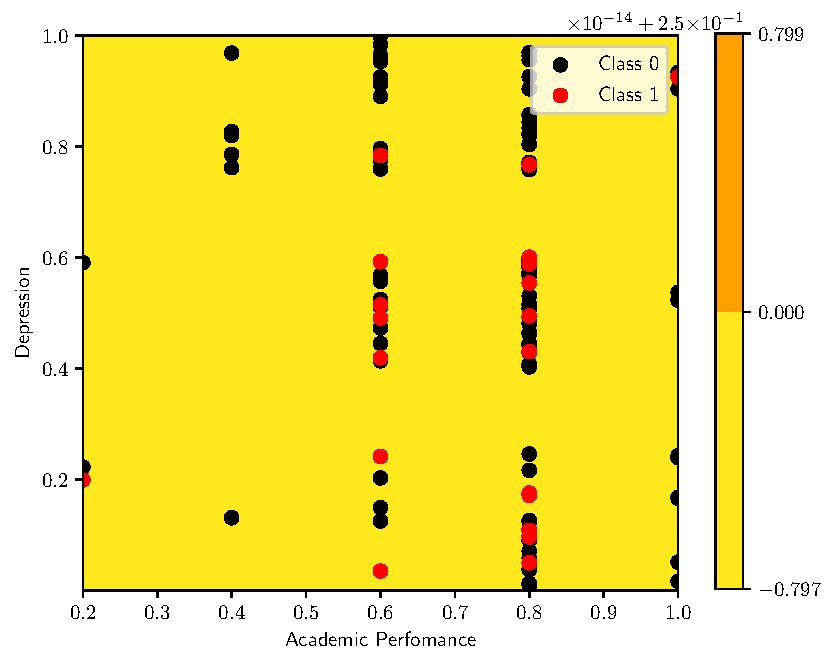
\includegraphics[width=\textwidth]{figs/tree-contour-1-3.pdf}
    \caption{}
  \end{subfigure}
  \begin{subfigure}[b]{0.32\textwidth}
    \centering 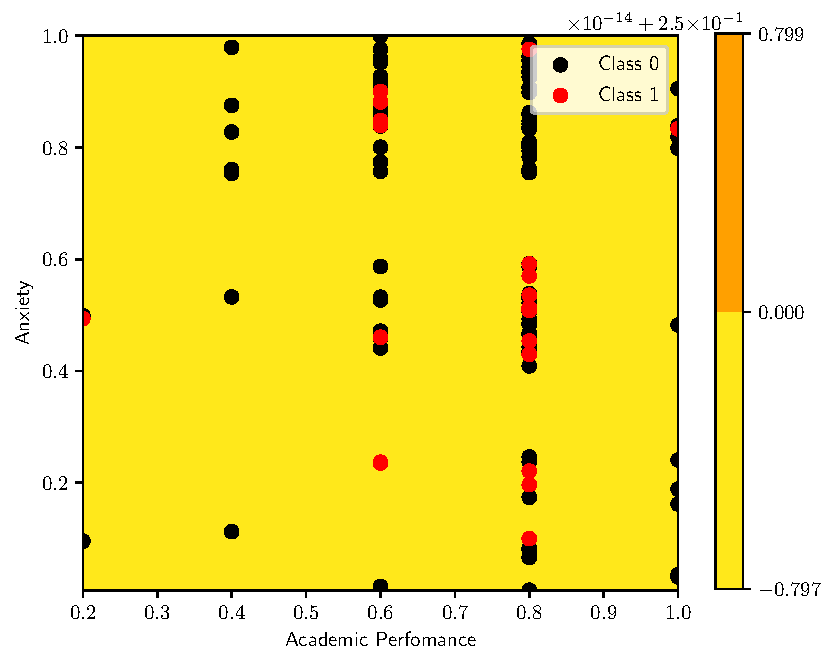
\includegraphics[width=\textwidth]{figs/tree-contour-1-4.pdf}
    \caption{}
  \end{subfigure}
  \begin{subfigure}[b]{0.32\textwidth}
    \centering 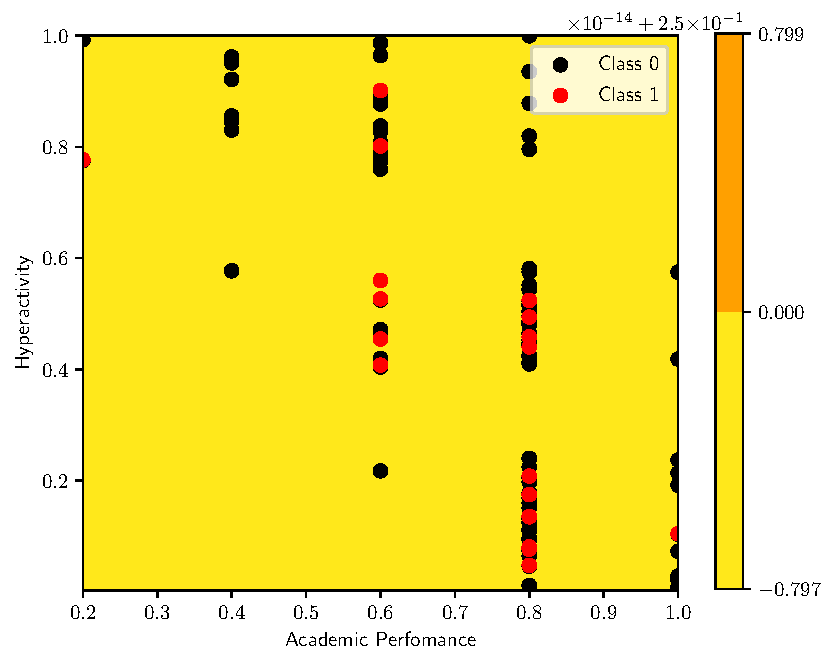
\includegraphics[width=\textwidth]{figs/tree-contour-1-5.pdf}
    \caption{}
  \end{subfigure}

  \begin{subfigure}[b]{0.32\textwidth}
    \centering 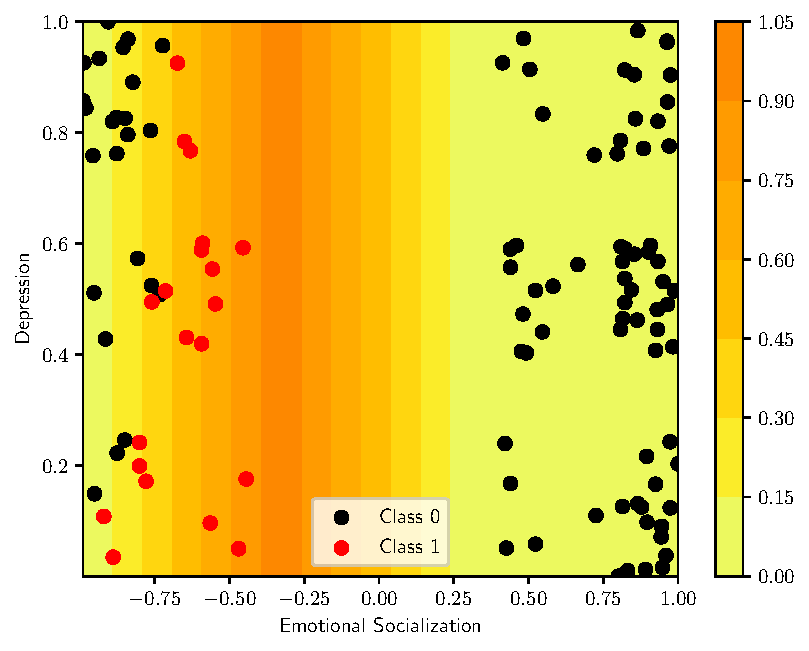
\includegraphics[width=\textwidth]{figs/tree-contour-2-3.pdf}
    \caption{}
  \end{subfigure}
  \begin{subfigure}[b]{0.32\textwidth}
    \centering 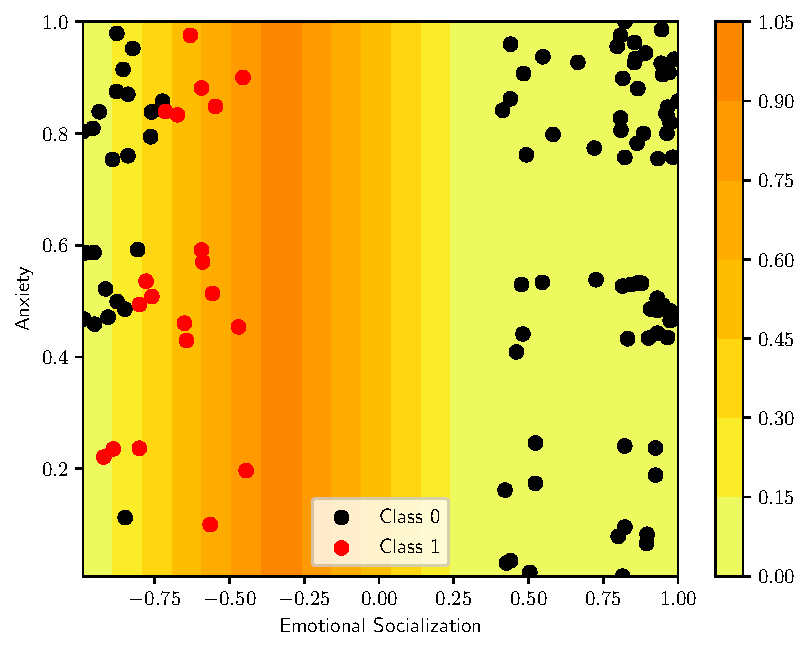
\includegraphics[width=\textwidth]{figs/tree-contour-2-4.pdf}
    \caption{}
  \end{subfigure}
  \begin{subfigure}[b]{0.32\textwidth}
    \centering 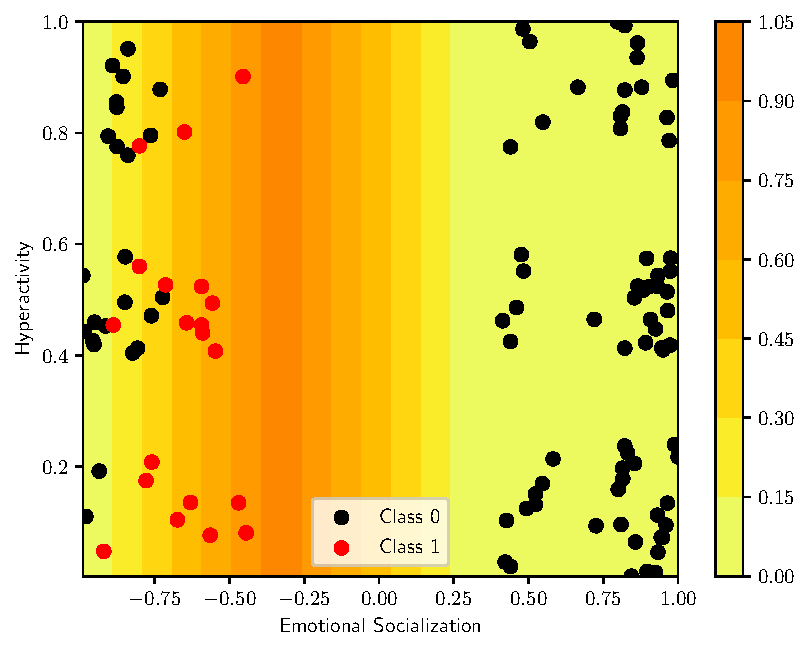
\includegraphics[width=\textwidth]{figs/tree-contour-2-5.pdf}
    \caption{}
  \end{subfigure}
  \caption{Decision Tree contour with real labels.}
  \label{fig:dts}
\end{figure*}

